% Provenance (never printed): cycle 4 SVT, "La planete Terre": the dynamics of
% the Earth's outer shell, plates and their boundaries, continental drift as a
% history of ideas; see sources/outline_sources.md. Pilot chapter, 2026-10-22.
\chapter{Platentektoniek: de bewegende puzzel}\label{ch:g7:plate-tectonics}

Spreid een \omterm{def:g3:continents-and-oceans:world-map}{wereldkaart} uit op tafel en kijk naar de twee \omterm{def:g1:landscapes-around-us:water}{kusten} van de
Atlantische \omterm{def:g2:water-on-earth:ocean}{Oceaan}. De grote bolling van Brazilië lijkt gemaakt om in de
holte van de westkust van Afrika te schuiven, alsof iemand één stuk land
in tweeën had gesneden en de helften uit elkaar had geduwd. De eersten die
goede \omterm{def:g2:drawing-to-map:map}{kaarten} van beide \omterm{def:g1:landscapes-around-us:water}{kusten} drukten, zagen het meteen. Drie eeuwen lang
bleef het een curiositeit. In de twintigste eeuw werd het het beginpunt
van de theorie die nu verklaart waarom de grond in Japan schudt, waarom de
Andes zo hoog zijn, waarom IJsland langzaam breder wordt --- en waarom de
\omterm{def:g2:drawing-to-map:map}{kaart} op tafel maar een momentopname is van een wereld die beweegt.

\begin{omfigure}
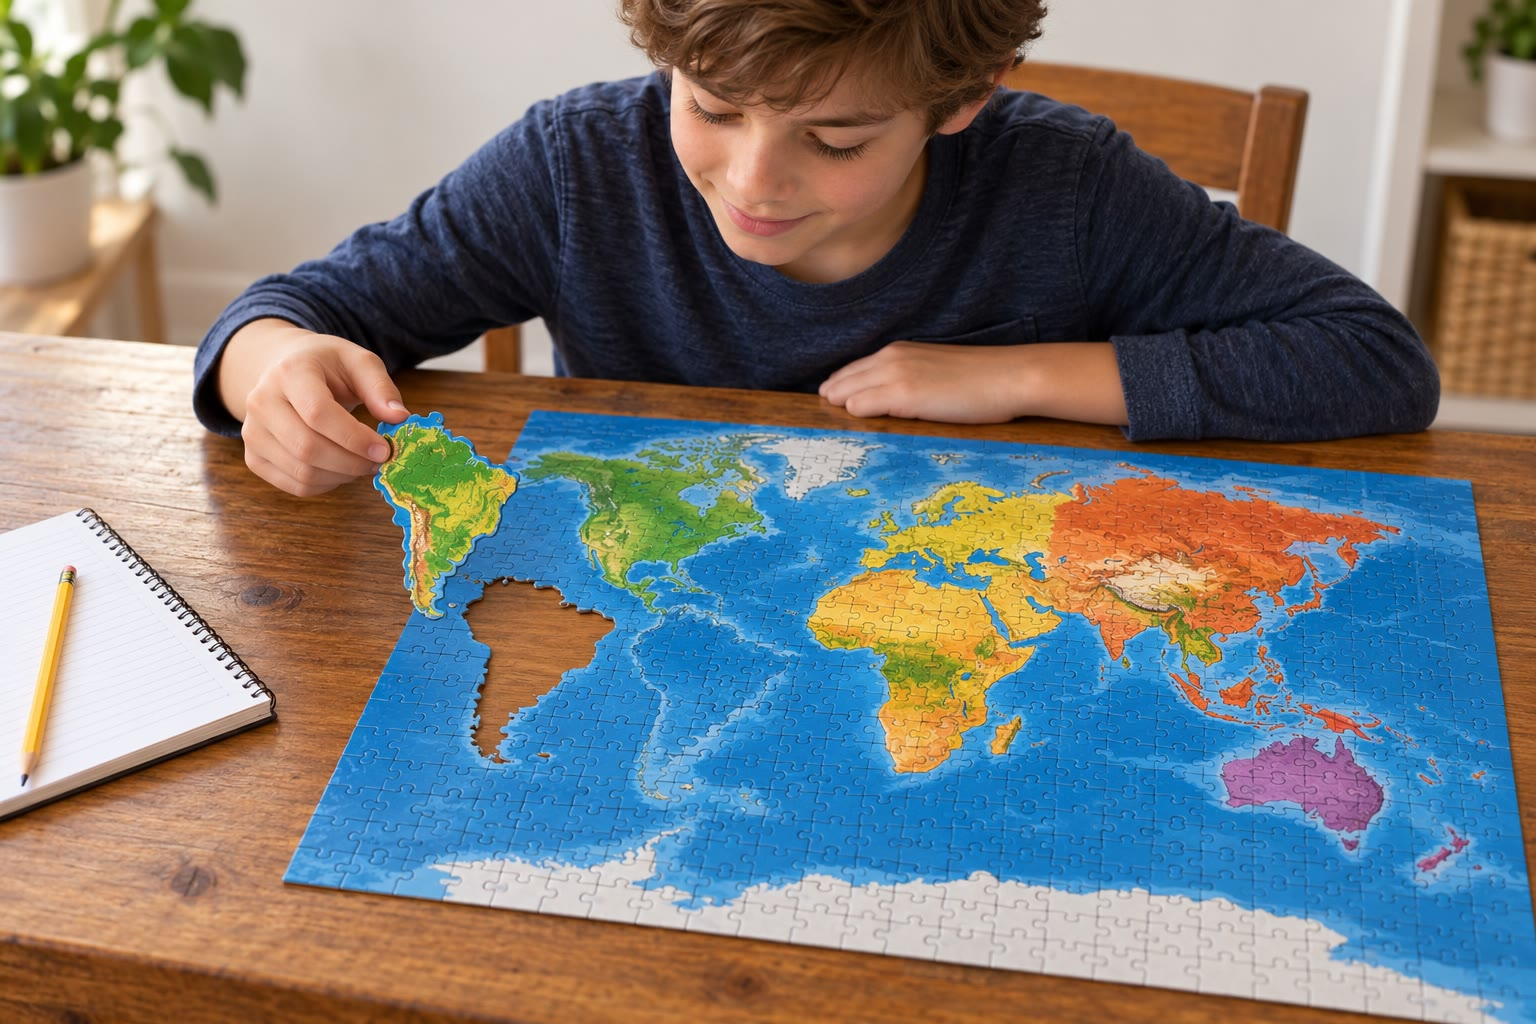
\includegraphics[width=0.62\linewidth]{images/book1/ai/g7-puzzle-map.jpg}

{\small Zuid-Amerika naast Afrika: in een puzzel is het passen een
spelletje; op de echte Aarde is het een aanwijzing.}
\end{omfigure}

\begin{recall}
De Aarde heeft drie hoofdlagen: een dunne \emph{\omterm{def:g6:inside-the-earth:layers}{aardkorst}} van \omterm{def:g3:stones-pebbles-sand:rock}{gesteente},
een dikke \emph{\omterm{def:g6:inside-the-earth:layers}{mantel}} van heet \omterm{def:g3:stones-pebbles-sand:rock}{gesteente} en een metalen \emph{\omterm{def:g6:inside-the-earth:layers}{kern}}; de
temperatuur stijgt met de diepte (\cref{ch:g6:inside-the-earth}). Een
plaats op de \omterm{def:g3:continents-and-oceans:globe}{globe} wordt bepaald door haar \omterm{def:g6:latitude-longitude:latitude}{breedtegraad} en haar
\omterm{def:g6:latitude-longitude:longitude}{lengtegraad} (\cref{ch:g6:latitude-longitude}).
\end{recall}

\section{Continenten die ooit in elkaar pasten}

\begin{definition}[Continentverschuiving]\label{def:g7:plate-tectonics:continental-drift}
\emph{Continentverschuiving}\index{continentverschuiving} is het idee dat
de \omterm{def:g3:continents-and-oceans:continent}{continenten} langzaam over het aardoppervlak bewegen, zodat hun plaats,
en de vorm van de \omterm{def:g2:water-on-earth:ocean}{oceanen} ertussen, in de loop van de tijd veranderd zijn.
\end{definition}

\begin{definition}[Supercontinent]\label{def:g7:plate-tectonics:supercontinent}
Een \emph{supercontinent}\index{supercontinent} is één landmassa die bestaat
uit alle, of bijna alle, \omterm{def:g3:continents-and-oceans:continent}{continenten} samen. Het laatste,
\emph{Pangea}\index{Pangea} (``alle landen'' in het Grieks), begon tussen
ongeveer 225 en 200 miljoen jaar geleden uiteen te vallen.
% ledger: usgs:pangaea-breakup
\end{definition}

De wetenschapper die \omterm{def:g7:plate-tectonics:continental-drift}{continentverschuiving} verdedigde als een echte
theorie, met bewijzen, was Alfred Wegener. Hij verzamelde vier soorten
aanwijzingen.

\begin{enumerate}
  \item \textbf{De vorm van de \omterm{def:g1:landscapes-around-us:water}{kusten}.} Zuid-Amerika en Afrika passen in
        elkaar als twee stukjes van een legpuzzel, en dat geldt ook voor
        een aantal andere kustlijnen.
  \item \textbf{Fossielen.} Dezelfde fossiele dieren en planten worden
        gevonden op \omterm{def:g3:continents-and-oceans:continent}{continenten} die nu door duizenden kilometers \omterm{def:g2:water-on-earth:ocean}{oceaan}
        gescheiden zijn. \emph{Mesosaurus} was een klein reptiel dat in \omterm{def:g2:water-on-earth:salt-fresh}{zoet
        water} leefde: het kan geen \omterm{def:g2:water-on-earth:ocean}{oceaan} zijn overgezwommen, maar toch
        liggen zijn fossielen zowel in Brazilië als in zuidelijk Afrika.
  \item \textbf{\omterm{def:g3:stones-pebbles-sand:rock}{Gesteenten}.} \omterm{def:g3:stones-pebbles-sand:rock}{Gesteenten} van dezelfde soort en dezelfde
        ouderdom, en oude \omterm{def:g4:world-physical-map:range}{gebergten} met dezelfde vorm, stoppen aan de ene
        \omterm{def:g1:landscapes-around-us:water}{kust} en gaan verder aan de overkant, zoals de regels op een
        gescheurde krant.
  \item \textbf{Klimaten van vroeger.} Steenkool, gemaakt van de planten van
        warme, moerassige bossen, wordt gevonden op Antarctica; sporen van
        vroegere gletsjers worden gevonden in delen van Afrika die nu heet
        en droog zijn. Deze landen moeten ooit in andere klimaten hebben
        gelegen, op andere breedtegraden.
\end{enumerate}
% ledger: usgs:coal-antarctica, usgs:fossil-map

\begin{omfigure}
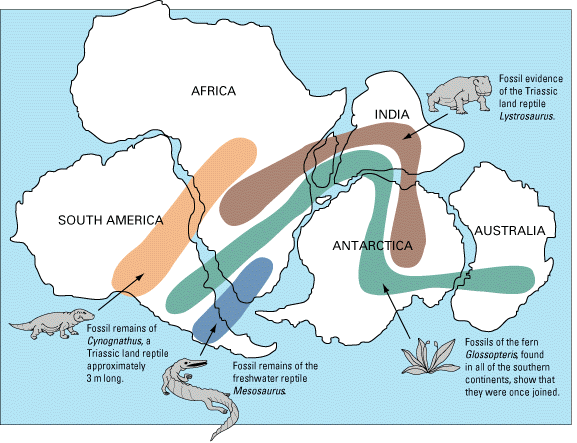
\includegraphics[width=0.86\linewidth]{images/book1/g7-usgs-fossil-map.png}

{\small De zuidelijke \omterm{def:g3:continents-and-oceans:continent}{continenten} weer in elkaar gezet. Elke gekleurde band
verbindt de plaatsen waar nu één fossiele soort wordt gevonden: de
landreptielen \emph{Cynognathus} en \emph{Lystrosaurus}, het
zoetwaterreptiel \emph{Mesosaurus} en de varen \emph{Glossopteris}. Als de
\omterm{def:g3:continents-and-oceans:continent}{continenten} uit elkaar liggen, raken de banden verspreid; als ze aan elkaar
liggen, lopen de banden zonder onderbreking door. \omterm{def:g2:drawing-to-map:map}{Kaart}: U.S. Geological
Survey, \emph{This Dynamic Earth} (publiek domein).}
\end{omfigure}

\begin{history}[Het idee van Wegener, 1912--1930]
% ledger: usgs:wegener-1912, usgs:wegener-death, usgs:jeffreys
Alfred Wegener, een 32-jarige Duitse meteoroloog, zette de theorie van de
\omterm{def:g7:plate-tectonics:continental-drift}{continentverschuiving} in 1912 uiteen in twee artikelen. De meeste geologen
verwierpen haar. Het sterkste bezwaar was dat Wegener niet kon zeggen
\emph{wat} de \omterm{def:g3:continents-and-oceans:continent}{continenten} bewoog: hij dacht dat ze door het \omterm{def:g3:stones-pebbles-sand:rock}{gesteente} van
de oceaanbodem ploegden, en de natuurkundige Harold Jeffreys liet zien dat
vaste \omterm{def:g3:continents-and-oceans:continent}{continenten} dat niet konden zonder te breken. Wegener bleef bewijzen
verzamelen tot hij in 1930 tijdens een expeditie op de ijskap van Groenland
stierf. Het antwoord dat hij miste, kwam van de bodem van de \omterm{def:g2:water-on-earth:ocean}{oceanen}, die
na de jaren 1950 werd verkend: dat wordt in een later jaar verteld.
\end{history}

\section{De platen}

De aanwijzingen van Wegener klopten, maar zijn \omterm{def:g3:continents-and-oceans:continent}{continenten} waren de
verkeerde stukken. Niet alleen de \omterm{def:g3:continents-and-oceans:continent}{continenten} bewegen: de hele buitenste
schil van de Aarde, onder de \omterm{def:g3:continents-and-oceans:continent}{continenten} en onder de \omterm{def:g2:water-on-earth:ocean}{oceanen}, is in stukken
gebroken.

\begin{definition}[Tektonische plaat]\label{def:g7:plate-tectonics:plate}
Een \emph{tektonische plaat}\index{tektonische plaat} (of gewoon een plaat)
is een grote, stijve schol van \omterm{def:g3:stones-pebbles-sand:rock}{gesteente} die deel uitmaakt van de buitenste
schil van de Aarde. Een plaat bestaat uit de \omterm{def:g6:inside-the-earth:layers}{aardkorst} en uit het
bovenste, koude en stijve deel van de \omterm{def:g6:inside-the-earth:layers}{mantel}, samen gemiddeld minstens
80 kilometer dik; ze beweegt langzaam over de hetere en zachtere \omterm{def:g6:inside-the-earth:layers}{mantel}
eronder.
% ledger: usgs:lithosphere-80km
\end{definition}

\begin{definition}[Platentektoniek]\label{def:g7:plate-tectonics:plate-tectonics}
\emph{Platentektoniek}\index{platentektoniek} is de theorie dat de buitenste
schil van de Aarde is verdeeld in \omterm{def:g7:plate-tectonics:plate}{platen} die ten opzichte van elkaar
bewegen, en dat de meeste \omterm{def:g4:volcanoes-earthquakes-first-look:earthquake}{aardbevingen}, \omterm{def:g4:volcanoes-earthquakes-first-look:volcano}{vulkanen} en \omterm{def:g4:world-physical-map:range}{gebergten} ontstaan waar
\omterm{def:g7:plate-tectonics:plate}{platen} elkaar ontmoeten.
\end{definition}

\begin{remark}[Hoeveel platen?]\label{rem:g7:plate-tectonics:how-many}
% ledger: usgs:plates-dozen, pb2002:count
Ongeveer een dozijn \omterm{def:g7:plate-tectonics:plate}{platen} is groot; veel meer zijn klein. Een
gedetailleerde \omterm{def:g2:drawing-to-map:map}{kaart} die geologen gebruiken, telt er 52. Een \omterm{def:g7:plate-tectonics:plate}{plaat} kan een
\omterm{def:g3:continents-and-oceans:continent}{continent} dragen, een \omterm{def:g2:water-on-earth:ocean}{oceaan}, of allebei: de Zuid-Amerikaanse \omterm{def:g7:plate-tectonics:plate}{plaat} draagt
heel Zuid-Amerika en de westelijke helft van het zuiden van de Atlantische
\omterm{def:g2:water-on-earth:ocean}{Oceaan}. De Pacifische \omterm{def:g7:plate-tectonics:plate}{plaat}, de grootste, draagt bijna helemaal geen land.
\end{remark}

\begin{omfigure}
\begin{tikzpicture}
\begin{axis}[ommap, width=\linewidth, xtick={-180,-90,...,180}, ytick={-60,0,60}]
\addplot[fill=omLithAlluv, draw=black!45, line width=0.2pt] table {figdata/out/shared-geo-land.dat};
\addplot[omRidge, line width=0.8pt] table {figdata/out/shared-geo-school-ridge.dat};
\addplot[omRidge!70!black, line width=0.8pt] table {figdata/out/shared-geo-school-transform.dat};
\addplot[omTrench, line width=0.8pt] table {figdata/out/shared-geo-school-subduction.dat};
\addplot[fill=omTrench, draw=none] table {figdata/out/shared-geo-school-teeth.dat};
\addplot[black!65, line width=0.8pt] table {figdata/out/shared-geo-school-collision.dat};
\begin{scope}[every node/.style={font=\scriptsize\bfseries, text=black!85,
    fill=white, fill opacity=0.75, text opacity=1, inner sep=1pt, align=center}]
  \node at (axis cs:-150,12) {Pacifische};
  \node at (axis cs:-103,52) {Noord-\\Amerikaanse};
  \node at (axis cs:-48,-12) {Zuid-\\Amerikaanse};
  \node at (axis cs:85,57) {Euraziatische};
  \node at (axis cs:18,8) {Afrikaanse};
  \node at (axis cs:10,-75) {Antarctische};
  \node at (axis cs:78,11) {Indische};
  \node at (axis cs:128,-26) {Australische};
  \node at (axis cs:-95,-22) {Nazca};
  \node at (axis cs:50,20) {Arabische};
\end{scope}
\end{axis}
\end{tikzpicture}

{\small De belangrijkste tektonische \omterm{def:g7:plate-tectonics:plate}{platen}. Rood: \omterm{def:g7:plate-tectonics:plate}{platen} die uit elkaar
bewegen; blauw met driehoekjes: de ene \omterm{def:g7:plate-tectonics:plate}{plaat} zakt onder de andere (de
driehoekjes staan op de \omterm{def:g7:plate-tectonics:plate}{plaat} die boven blijft); grijs: \omterm{def:g7:plate-tectonics:plate}{platen} die tegen
elkaar duwen over een brede zone van \omterm{def:g4:world-physical-map:range}{gebergten}; donkerrood: \omterm{def:g7:plate-tectonics:plate}{platen} die
langs elkaar schuiven. \omterm{def:g7:plate-tectonics:plate-boundary}{Plaatgrenzen} naar P.~Bird (2003); kustlijnen van
Natural Earth.}
\end{omfigure}

Hoe weten we waar de ene \omterm{def:g7:plate-tectonics:plate}{plaat} ophoudt en de volgende begint? Kijk waar de
Aarde onrustig is.

\begin{proposition}[Aardbevingen en vulkanen tekenen de plaatgrenzen]\label{prop:g7:plate-tectonics:restless}
% ledger: data:usgs-comcat, data:pb2002 (share computed in figdata/grade-7/quakes_on_boundaries.py)
\omterm{def:g4:volcanoes-earthquakes-first-look:earthquake}{Aardbevingen} en \omterm{def:g4:volcanoes-earthquakes-first-look:volcano}{vulkanen} liggen niet willekeurig verspreid over de Aarde:
de meeste liggen langs smalle gordels, en die gordels zijn de randen van de
\omterm{def:g7:plate-tectonics:plate}{platen}. Van de 7\,031 \omterm{def:g4:volcanoes-earthquakes-first-look:earthquake}{aardbevingen} met een magnitude van 6 of meer die
tussen 1976 en 2025 zijn geregistreerd, vonden er 6\,472 --- dat is
92\,\% --- plaats op minder dan \qty{300}{km} van een \omterm{def:g7:plate-tectonics:plate-boundary}{plaatgrens}.
\end{proposition}

\begin{omfigure}
\begin{tikzpicture}
\begin{axis}[ommap, width=\linewidth, xtick={-180,-90,...,180}, ytick={-60,0,60},
  legend style={at={(0.02,0.04)}, anchor=south west, font=\scriptsize,
  fill=white, fill opacity=0.85, text opacity=1, draw=black!40}]
\addplot[fill=omLithAlluv, draw=black!45, line width=0.2pt, forget plot] table {figdata/out/shared-geo-land.dat};
\addplot[only marks, mark=*, mark size=0.45pt, omThm!85!black] table[x=lon, y=lat] {figdata/out/grade-7-quakes_on_boundaries-map.dat};
\addlegendentry{aardbeving, magnitude 6.5 of meer, 1976--2025}
\addplot[only marks, mark=triangle*, mark size=1.1pt, black] table {figdata/out/shared-geo-volcanoes.dat};
\addlegendentry{vulkaan actief in de laatste 12\,000 jaar}
\end{axis}
\end{tikzpicture}

{\small Grote \omterm{def:g4:volcanoes-earthquakes-first-look:earthquake}{aardbevingen} en recente \omterm{def:g4:volcanoes-earthquakes-first-look:volcano}{vulkanen}. Vergelijk met de \omterm{def:g2:drawing-to-map:map}{kaart} van
de \omterm{def:g7:plate-tectonics:plate}{platen} hierboven: de stippen en de driehoekjes tekenen de \omterm{def:g7:plate-tectonics:plate-boundary}{plaatgrenzen}.
Gegevens: aardbevingscatalogus van de U.S. Geological Survey; Smithsonian
Global Volcanism Program.}
\end{omfigure}

\section{Drie soorten plaatgrenzen}

\begin{definition}[Plaatgrens]\label{def:g7:plate-tectonics:plate-boundary}
Een \emph{plaatgrens}\index{plaatgrens} is de lijn, of de smalle zone,
waar twee \omterm{def:g7:plate-tectonics:plate}{platen} elkaar ontmoeten. Naar de manier waarop de twee \omterm{def:g7:plate-tectonics:plate}{platen}
ten opzichte van elkaar bewegen, is een plaatgrens van een van drie
soorten:
\begin{itemize}
  \item bij een \emph{divergente grens}\index{divergente grens} bewegen de
        twee \omterm{def:g7:plate-tectonics:plate}{platen} uit elkaar;
  \item bij een \emph{convergente grens}\index{convergente grens} bewegen de
        twee \omterm{def:g7:plate-tectonics:plate}{platen} naar elkaar toe;
  \item bij een \emph{transforme grens}\index{transforme grens} schuiven de
        twee \omterm{def:g7:plate-tectonics:plate}{platen} zij aan zij langs elkaar.
\end{itemize}
\end{definition}

\begin{example}[Divergente grenzen: IJsland en Oost-Afrika]\label{ex:g7:plate-tectonics:divergent}
% ledger: usgs:iceland, usgs:east-africa
Midden door de Atlantische \omterm{def:g2:water-on-earth:ocean}{Oceaan} loopt een keten van onderzeese \omterm{def:g1:landscapes-around-us:landform}{bergen},
de Midden-Atlantische Rug, waar de \omterm{def:g7:plate-tectonics:plate}{platen} aan weerszijden uit elkaar
bewegen. Heet \omterm{def:g3:stones-pebbles-sand:rock}{gesteente} uit de \omterm{def:g6:inside-the-earth:layers}{mantel} stijgt op in de opening, smelt
gedeeltelijk en wordt nieuwe zeebodem: een \omterm{def:g7:plate-tectonics:plate-boundary}{divergente grens} bouwt nieuwe
\omterm{def:g7:plate-tectonics:plate}{plaat}. IJsland is een stuk van deze rug dat boven de \omterm{def:g2:water-on-earth:ocean}{zee} uitsteekt: daar
beweegt Noord-Amerika naar het westen en Eurazië naar het oosten, en wordt
het eiland langzaam opengescheurd. Tussen 1975 en 1984 werden de spleten
bij de \omterm{def:g4:volcanoes-earthquakes-first-look:volcano}{vulkaan} Krafla, in het noorden van het eiland, in totaal ongeveer
7 meter wijder. Een \omterm{def:g7:plate-tectonics:plate-boundary}{divergente grens} kan ook door een \omterm{def:g3:continents-and-oceans:continent}{continent} lopen:
langs de Oost-Afrikaanse Slenk begint Afrika te splijten, en de Rode \omterm{def:g2:water-on-earth:ocean}{Zee} is
een jonge \omterm{def:g2:water-on-earth:ocean}{oceaan} die Arabië al van Afrika heeft gescheiden.
\end{example}

\begin{example}[Convergente grenzen: de Andes en de Himalaya]\label{ex:g7:plate-tectonics:convergent}
% ledger: usgs:trench-depth, usgs:himalaya
Voor de westkust van Zuid-Amerika beweegt de Nazcaplaat, die \omterm{def:g2:water-on-earth:ocean}{oceaan}
draagt, naar de Zuid-Amerikaanse \omterm{def:g7:plate-tectonics:plate}{plaat} toe, die een \omterm{def:g3:continents-and-oceans:continent}{continent} draagt. De
oceanische \omterm{def:g7:plate-tectonics:plate}{plaat}, die zwaarder is, buigt en zakt onder het \omterm{def:g3:continents-and-oceans:continent}{continent}, diep
de \omterm{def:g6:inside-the-earth:layers}{mantel} in. Langs de lijn waar ze naar beneden gaat, duikt de zeebodem
weg in een diepe trog; boven de zakkende \omterm{def:g7:plate-tectonics:plate}{plaat} wordt het land geschud door
\omterm{def:g4:volcanoes-earthquakes-first-look:earthquake}{aardbevingen} en staan er rijen \omterm{def:g4:volcanoes-earthquakes-first-look:volcano}{vulkanen}: de Andes. In het westen van de
Stille \omterm{def:g2:water-on-earth:ocean}{Oceaan}, waar de ene oceanische \omterm{def:g7:plate-tectonics:plate}{plaat} onder een andere zakt, liggen
de troggen die de diepste plaatsen op Aarde zijn: de Marianentrog is bijna
\qty{11000}{m} diep. Als twee \omterm{def:g3:continents-and-oceans:continent}{continenten} elkaar ontmoeten, zakt geen van
beide: de korst wordt samengedrukt en dikker. India botste ongeveer
50 miljoen jaar geleden met Azië, en de twee \omterm{def:g7:plate-tectonics:plate}{platen} duwen nog steeds; zo
zijn de Himalaya en het Hoogland van Tibet omhooggekomen.
\end{example}

\begin{example}[Een transforme grens: de San Andreasbreuk]\label{ex:g7:plate-tectonics:transform}
% ledger: usgs:san-andreas, usgs:san-andreas-photo
In Californië schuift de Pacifische \omterm{def:g7:plate-tectonics:plate}{plaat} naar het noordwesten langs de
Noord-Amerikaanse \omterm{def:g7:plate-tectonics:plate}{plaat}, langs de San Andreasbreuk, die ongeveer
\qty{1300}{km} lang is. Daar wordt geen \omterm{def:g7:plate-tectonics:plate}{plaat} gemaakt of vernietigd; de twee
\omterm{def:g7:plate-tectonics:plate}{platen} schuren langs elkaar, en de schokken van dat schuren zijn
\omterm{def:g4:volcanoes-earthquakes-first-look:earthquake}{aardbevingen}.
\end{example}

\begin{omfigure}
\begin{tikzpicture}[x=1cm, y=1cm, font=\small]
  % mantle
  \fill[omLithGranite!45] (0,-3.3) rectangle (12.4,-0.85);
  \node[font=\footnotesize, text=black!75] at (2.6,-2.6) {mantel: heet en zacht};
  % sea water
  \fill[omSea] (0,0) -- (0,-0.75) -- (1.5,-0.6) -- (3,-0.25) -- (4.5,-0.6)
    -- (7.4,-0.8) -- (8.0,-1.2) -- (8.6,-0.6) -- (8.9,0) -- cycle;
  % oceanic plates (the ridge at x = 3, the trench at x = 8)
  \fill[omLithBasalt!70] (0,-0.75) -- (1.5,-0.6) -- (3,-0.25) -- (4.5,-0.6)
    -- (7.4,-0.8) -- (8.0,-1.2) -- (9.6,-2.3) -- (10.2,-3.3) -- (9.5,-3.3)
    -- (8.6,-2.2) -- (7.5,-1.55) -- (4.5,-1.35) -- (3.2,-0.95) -- (2.8,-0.95)
    -- (1.5,-1.35) -- (0,-1.45) -- cycle;
  % continental plate
  \fill[omLithSand!80] (8.6,-0.6) -- (8.9,0) -- (9.4,0.35) -- (9.8,0.9)
    -- (10.2,0.35) -- (12.4,0.2) -- (12.4,-1.9) -- (10.6,-1.9) -- (9.6,-2.3)
    -- (8.0,-1.2) -- cycle;
  \draw[black!70, line width=0.5pt] (0,-0.75) -- (1.5,-0.6) -- (3,-0.25)
    -- (4.5,-0.6) -- (7.4,-0.8) -- (8.0,-1.2) -- (8.6,-0.6) -- (8.9,0)
    -- (9.4,0.35) -- (9.8,0.9) -- (10.2,0.35) -- (12.4,0.2);
  \draw[black!45, densely dashed] (0,0) -- (8.9,0);
  % magma: under the ridge and under the volcano
  \fill[omThm!80] (2.85,-0.95) -- (3,-0.3) -- (3.15,-0.95) -- cycle;
  \draw[omThm!80, line width=1.4pt, -{Stealth[length=2.2mm]}] (3,-1.85) -- (3,-1.0);
  \draw[omThm!80, line width=1.2pt, decorate, decoration={snake, amplitude=0.6pt,
    segment length=4pt}] (9.8,-2.45) -- (9.8,0.75);
  % plate motions
  \draw[black, line width=1pt, -{Stealth[length=2.4mm]}] (2.5,-0.75) -- (1.3,-0.95);
  \draw[black, line width=1pt, -{Stealth[length=2.4mm]}] (3.5,-0.75) -- (5.4,-1.05);
  \draw[black, line width=1pt, -{Stealth[length=2.4mm]}] (12.1,-0.85) -- (10.9,-0.85);
  \draw[black, line width=1pt, -{Stealth[length=2.4mm]}] (8.7,-1.75) -- (9.3,-2.25);
  % labels
  \node[font=\footnotesize, align=center, above] at (3,0.05) {divergente grens:\\oceanische rug};
  \node[font=\footnotesize, align=center, below] at (6.9,-1.95) {convergente grens:\\de oceanische plaat zakt};
  \draw[black!60, thin] (8.0,-1.25) -- (7.6,-1.9);
  \node[font=\footnotesize, above] at (8.0,0.05) {trog};
  \draw[black!60, thin] (8.0,0.05) -- (8.0,-1.1);
  \node[font=\footnotesize, above] at (9.8,0.95) {vulkaan};
  \node[font=\footnotesize] at (11.4,-0.4) {continent};
  \node[font=\footnotesize] at (1.2,-1.6) {oceanische plaat};
  \node[font=\footnotesize, text=black!70] at (5.6,-0.32) {oceaan};
\end{tikzpicture}

\medskip
\begin{tikzpicture}[font=\small]
  \fill[omLithBasalt!45] (0,0) rectangle (2.4,2.2);
  \fill[omLithSand!70] (2.4,0) rectangle (4.8,2.2);
  \draw[fault] (2.4,-0.1) -- (2.4,2.3);
  \draw[black, line width=1pt, -{Stealth[length=2.4mm]}] (1.2,0.5) -- (1.2,1.7);
  \draw[black, line width=1pt, -{Stealth[length=2.4mm]}] (3.6,1.7) -- (3.6,0.5);
  \node[font=\footnotesize, below] at (1.2,-0.1) {plaat A};
  \node[font=\footnotesize, below] at (3.6,-0.1) {plaat B};
  \node[font=\footnotesize, align=left, anchor=west] at (5.1,1.1)
    {transforme grens, van bovenaf gezien:\\de platen schuiven langs elkaar;\\er wordt geen plaat gemaakt of vernietigd};
\end{tikzpicture}

{\small Boven: een doorsnede door twee \omterm{def:g7:plate-tectonics:plate-boundary}{plaatgrenzen} (niet op schaal; de
diepten zijn sterk overdreven). Bij de rug bewegen de \omterm{def:g7:plate-tectonics:plate}{platen} uit elkaar en
stijgt heet \omterm{def:g3:stones-pebbles-sand:rock}{gesteente} op uit de \omterm{def:g6:inside-the-earth:layers}{mantel}; bij de trog zakt de oceanische
\omterm{def:g7:plate-tectonics:plate}{plaat} onder het \omterm{def:g3:continents-and-oceans:continent}{continent}, en het \omterm{def:g3:stones-pebbles-sand:rock}{gesteente} dat erboven smelt, voedt
\omterm{def:g4:volcanoes-earthquakes-first-look:volcano}{vulkanen}. Onder: een \omterm{def:g7:plate-tectonics:plate-boundary}{transforme grens} van bovenaf gezien.}
\end{omfigure}

\begin{omfigure}
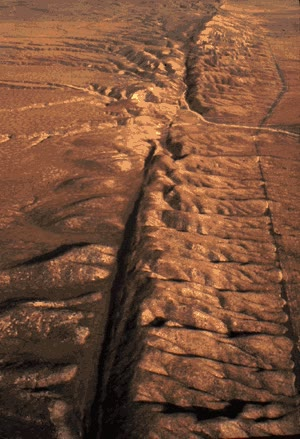
\includegraphics[width=0.28\linewidth]{images/book1/g7-usgs-san-andreas.jpg}

{\small De San Andreasbreuk dwars door de Carrizo Plain, Californië, gezien
vanuit een vliegtuig: het lange rechte \omterm{def:g1:landscapes-around-us:landform}{dal} is de grens tussen de
Pacifische \omterm{def:g7:plate-tectonics:plate}{plaat} (links) en de Noord-Amerikaanse \omterm{def:g7:plate-tectonics:plate}{plaat} (rechts). Foto:
Robert E. Wallace, U.S. Geological Survey (publiek domein).}
\end{omfigure}

\begin{method}[Een plaatgrens op een kaart herkennen]\label{met:g7:plate-tectonics:recognise}
Om te bepalen wat voor grens twee \omterm{def:g7:plate-tectonics:plate}{platen} scheidt:
\begin{enumerate}
  \item zoek op een \omterm{def:g2:drawing-to-map:map}{kaart} van de plaatbewegingen de pijlen aan weerszijden
        van de grens;
  \item als ze van de grens af wijzen, is die divergent; als ze ernaartoe
        wijzen, convergent; als ze evenwijdig aan de grens lopen en in
        tegengestelde richtingen wijzen, transform;
  \item controleer met het \omterm{def:g1:landscapes-around-us:landscape}{landschap}: een rug midden in een \omterm{def:g2:water-on-earth:ocean}{oceaan} of een
        slenk dwars door een \omterm{def:g3:continents-and-oceans:continent}{continent} hoort bij een \omterm{def:g7:plate-tectonics:plate-boundary}{divergente grens}; een
        diepe trog met een rij \omterm{def:g4:volcanoes-earthquakes-first-look:volcano}{vulkanen}, of een hoog \omterm{def:g4:world-physical-map:range}{gebergte}, bij een
        convergente; een lange rechte breuk zonder het een of het ander bij
        een \omterm{def:g7:plate-tectonics:plate-boundary}{transforme grens}.
\end{enumerate}
\end{method}

\section{Hoe snel bewegen platen?}

\begin{proposition}[Een paar centimeter per jaar]\label{prop:g7:plate-tectonics:speed}
% ledger: data:pb2002 (speeds computed in figdata/grade-7/plate_speeds.py), usgs:mar-rate
Twee naburige \omterm{def:g7:plate-tectonics:plate}{platen} bewegen ten opzichte van elkaar met een snelheid van
een paar centimeter per jaar: van ongeveer 2 centimeter per jaar in het
noorden van de Atlantische \omterm{def:g2:water-on-earth:ocean}{Oceaan} tot meer dan 14 centimeter per jaar bij
de Oost-Pacifische Rug, de rug die op Aarde het snelst uitspreidt.
\end{proposition}

\begin{omfigure}
\begin{tikzpicture}
\begin{axis}[xbar, width=0.82\linewidth, height=5.4cm, xmin=0, xmax=16.5,
  ytick={1,...,6}, yticklabels={Noord-Atlantische rug, Zuid-Atlantische rug,
  San Andreasbreuk, Himalaya, Peru-Chilitrog, Oost-Pacifische Rug},
  y tick label style={font=\small}, tick label style={font=\small},
  xlabel={snelheid van de ene plaat ten opzichte van de andere (cm per jaar)},
  label style={font=\small}, bar width=7pt, axis x line=bottom,
  axis y line=left, axis line style={-}, enlarge y limits=0.12,
  nodes near coords, nodes near coords style={font=\scriptsize},
  every node near coord/.append style={/pgf/number format/fixed,
  /pgf/number format/precision=1, /pgf/number format/fixed zerofill}]
\addplot[fill=omDef!55, draw=omDef!80!black] table[x=speed_cm_a, y=rank] {figdata/out/grade-7-plate_speeds.dat};
\end{axis}
\end{tikzpicture}

{\small Hoe snel \omterm{def:g7:plate-tectonics:plate}{platen} bewegen bij zes \omterm{def:g7:plate-tectonics:plate-boundary}{plaatgrenzen}: gemiddelden langs
elke grens, berekend uit het platenmodel van P.~Bird (2003).}
\end{omfigure}

\begin{method}[Van centimeter per jaar naar kilometer per miljoen jaar]\label{met:g7:plate-tectonics:convert}
Een kilometer is \num{100000} centimeter. Een snelheid van \qty{1}{cm} per
jaar, een miljoen jaar volgehouden, legt dus \num{1000000} centimeter af,
dat is \qty{10}{km}. Daarom:
\[
  1\ \text{cm per jaar} = 10\ \text{km per miljoen jaar}.
\]
Vermenigvuldig een snelheid in centimeter per jaar met 10 om kilometer per
miljoen jaar te krijgen; vermenigvuldig daarna met een aantal miljoenen
jaren om een afstand in kilometer te krijgen, of deel een afstand door de
snelheid om een tijd te krijgen.
\end{method}

\begin{example}[De Atlantische Oceaan groeit]\label{ex:g7:plate-tectonics:atlantic}
% ledger: usgs:mar-rate
Gemiddeld bewegen de twee kanten van de Midden-Atlantische Rug met ongeveer
\qty{2.5}{cm} per jaar uit elkaar, dat is \qty{25}{km} per miljoen jaar. In
100 miljoen jaar maakt dat \qty{2500}{km}: lang genoeg volgehouden opent
een snelheid die veel te traag is om in een mensenleven te merken een
\omterm{def:g2:water-on-earth:ocean}{oceaan}.
\end{example}

\begin{remark}[De beweging nu meten]\label{rem:g7:plate-tectonics:gps}
% ledger: usgs:gps
Zulke trage bewegingen worden nu rechtstreeks gemeten. Vaste meetstations
die op het \omterm{def:g3:stones-pebbles-sand:rock}{vaste gesteente} zijn bevestigd, ontvangen de signalen van
plaatsbepalingssatellieten en berekenen dag na dag hun eigen positie, tot
op een paar millimeter. Na een paar jaar zie je dat stations op
verschillende \omterm{def:g7:plate-tectonics:plate}{platen} uit elkaar gaan of naar elkaar toe komen, met de
snelheden die uit de \omterm{def:g3:stones-pebbles-sand:rock}{gesteenten} over miljoenen jaren zijn afgeleid.
Plaatsbepaling met satellieten zelf is het onderwerp van
\cref{ch:g9:maps-of-the-earth}.
\end{remark}

\begin{omfigure}
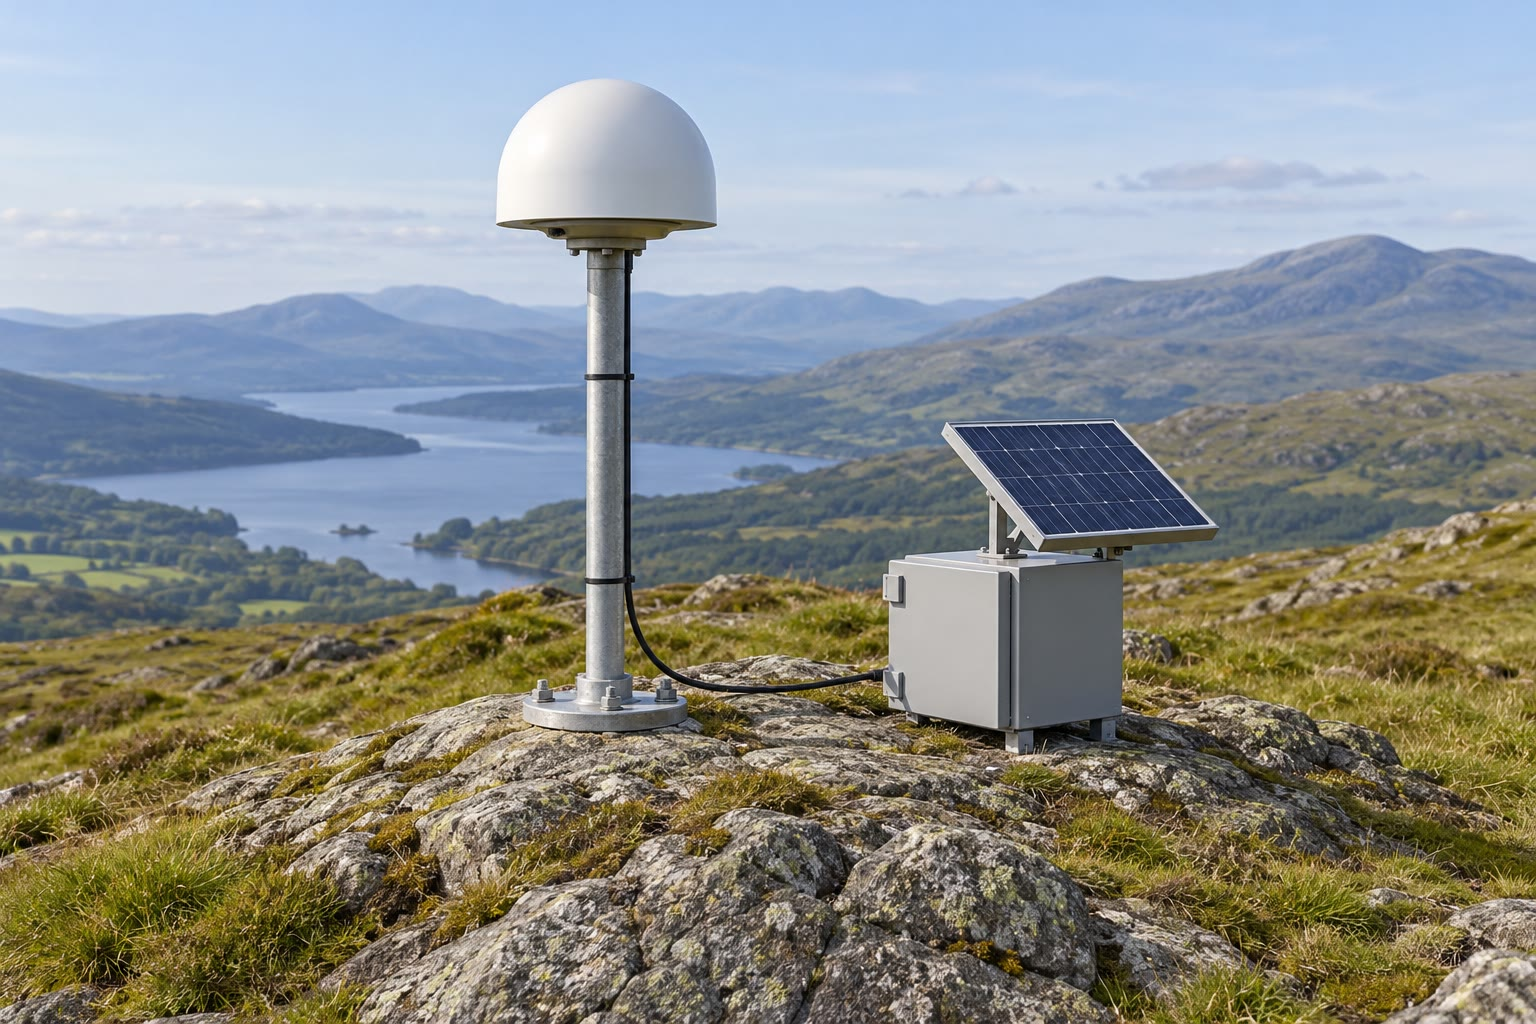
\includegraphics[width=0.55\linewidth]{images/book1/ai/g7-gps-station.jpg}

{\small Een vast meetstation voor plaatsbepaling: de antenne is aan het
\omterm{def:g3:stones-pebbles-sand:rock}{gesteente} vastgeschroefd, dus beweegt ze mee met de \omterm{def:g7:plate-tectonics:plate}{plaat}.}
\end{omfigure}

\section{Oefeningen}

\begin{exercise}[$\star$]\label{exo:g7:plate-tectonics:1}
Wat is \omterm{def:g7:plate-tectonics:continental-drift}{continentverschuiving}? Noem de vier soorten aanwijzingen die Wegener
gebruikte om haar te verdedigen.
\end{exercise}

\begin{exercise}[$\star$]\label{exo:g7:plate-tectonics:2}
Noem de drie soorten \omterm{def:g7:plate-tectonics:plate-boundary}{plaatgrenzen} en zeg voor elke soort hoe de twee
\omterm{def:g7:plate-tectonics:plate}{platen} ten opzichte van elkaar bewegen.
\end{exercise}

\begin{exercise}[$\star$]\label{exo:g7:plate-tectonics:3}
Kijk naar de \omterm{def:g2:drawing-to-map:map}{kaart} van de \omterm{def:g4:volcanoes-earthquakes-first-look:earthquake}{aardbevingen} en \omterm{def:g4:volcanoes-earthquakes-first-look:volcano}{vulkanen}. Noem twee gebieden in
de wereld met veel grote \omterm{def:g4:volcanoes-earthquakes-first-look:earthquake}{aardbevingen}, en één \omterm{def:g3:continents-and-oceans:continent}{continent} dat er in het
midden bijna geen heeft.
\end{exercise}

\begin{exercise}[$\star$]\label{exo:g7:plate-tectonics:4}
Fossielen van \emph{Mesosaurus}, een klein reptiel dat in \omterm{def:g2:water-on-earth:salt-fresh}{zoet water}
leefde, worden gevonden in Brazilië en in zuidelijk Afrika. Waarom is dit
een aanwijzing dat de twee \omterm{def:g3:continents-and-oceans:continent}{continenten} ooit aan elkaar vastzaten?
\end{exercise}

\begin{exercise}[$\star\star$]\label{exo:g7:plate-tectonics:5}
Er wordt steenkool gevonden op Antarctica. Wat zegt dit over het \omterm{def:g5:weather-and-climate:climate}{klimaat}
waarin de steenkool is ontstaan, en wat kunnen we concluderen over waar
Antarctica toen lag?
\end{exercise}

\begin{exercise}[$\star\star$]\label{exo:g7:plate-tectonics:6}
Zeg welke soort \omterm{def:g7:plate-tectonics:plate-boundary}{plaatgrens} er op elk van deze plaatsen ligt: de
Midden-Atlantische Rug; de Andes; de San Andreasbreuk; de Himalaya; de
Oost-Afrikaanse Slenk.
\end{exercise}

\begin{exercise}[$\star\star$]\label{exo:g7:plate-tectonics:7}
Zet een snelheid van \qty{2.5}{cm} per jaar om in kilometer per miljoen
jaar. Hoe ver zouden twee punten aan weerszijden van de grens met deze
snelheid in 60 miljoen jaar uit elkaar bewegen?
\end{exercise}

\begin{exercise}[$\star\star$]\label{exo:g7:plate-tectonics:8}
Tussen 1975 en 1984 --- negen jaar --- werden de spleten bij de \omterm{def:g4:volcanoes-earthquakes-first-look:volcano}{vulkaan}
Krafla in IJsland in totaal ongeveer \qty{7}{m} wijder. Hoeveel werden ze
gemiddeld per jaar wijder, in centimeter? Vergelijk dat met de gemiddelde
snelheid van de Midden-Atlantische Rug, ongeveer \qty{2.5}{cm} per jaar,
en bedenk waarom de twee getallen zo verschillen.
\end{exercise}

\begin{exercise}[$\star\star$]\label{exo:g7:plate-tectonics:9}
De theorie van Wegener werd tientallen jaren verworpen. Welke vraag kon hij
niet beantwoorden? Wat verandert de theorie van de \omterm{def:g7:plate-tectonics:plate-tectonics}{platentektoniek} aan zijn
beeld van bewegende \omterm{def:g3:continents-and-oceans:continent}{continenten}?
\end{exercise}

\begin{exercise}[$\star\star$]\label{exo:g7:plate-tectonics:10}
Kijk naar de doorsnede door twee \omterm{def:g7:plate-tectonics:plate-boundary}{plaatgrenzen}. Waar ligt de zeebodem het
hoogst, en waar het diepst? Waar wordt nieuwe \omterm{def:g7:plate-tectonics:plate}{plaat} gemaakt, en waar gaat
een \omterm{def:g7:plate-tectonics:plate}{plaat} terug de \omterm{def:g6:inside-the-earth:layers}{mantel} in?
\end{exercise}

\begin{exercise}[$\star\star\star$]\label{exo:g7:plate-tectonics:11}
Bij de Oost-Pacifische Rug bewegen de \omterm{def:g7:plate-tectonics:plate}{platen} met ongeveer \qty{14.2}{cm}
per jaar uit elkaar, en bij de Noord-Atlantische rug met ongeveer
\qty{2.2}{cm} per jaar. Hoeveel keer sneller is de Oost-Pacifische Rug
(afgerond op een heel getal)? Hoelang doet elke rug erover om
\qty{1000}{km} nieuwe oceaanbodem te openen?
\end{exercise}

\begin{exercise}[$\star\star\star$]\label{exo:g7:plate-tectonics:12}
% ledger: data:usgs-comcat, data:pb2002 (counts in figdata/grade-7/quakes_on_boundaries.py, part bands)
Van de 7\,031 \omterm{def:g4:volcanoes-earthquakes-first-look:earthquake}{aardbevingen} met een magnitude van 6 of meer die van 1976 tot
2025 zijn geregistreerd, vonden er 4\,578 plaats op minder dan
\qty{100}{km} van de lijn van een \omterm{def:g7:plate-tectonics:plate-boundary}{plaatgrens} op de \omterm{def:g2:drawing-to-map:map}{kaart}, 6\,472 op minder
dan \qty{300}{km} en 6\,786 op minder dan \qty{500}{km}.
(a) Hoeveel vonden er plaats tussen \qty{100}{km} en \qty{300}{km} van de
lijn? (b) Bereken, afgerond op een heel getal, het percentage van al deze
\omterm{def:g4:volcanoes-earthquakes-first-look:earthquake}{aardbevingen} dat op minder dan \qty{100}{km} van de lijn plaatsvond.
(c) Veel van de \omterm{def:g4:volcanoes-earthquakes-first-look:earthquake}{aardbevingen} tussen \qty{100}{km} en \qty{300}{km} van de
lijn liggen aan dezelfde kant van een diepe oceaantrog. Leg met wat er bij
een \omterm{def:g7:plate-tectonics:plate-boundary}{convergente grens} gebeurt uit waarom een \omterm{def:g4:volcanoes-earthquakes-first-look:earthquake}{aardbeving} die door een
\omterm{def:g7:plate-tectonics:plate-boundary}{plaatgrens} wordt veroorzaakt zo ver van de lijn op de \omterm{def:g2:drawing-to-map:map}{kaart} kan
plaatsvinden.
\end{exercise}

\section{Probleem: Het zuiden van de Atlantische Oceaan opent zich}

\begin{problem}[{Weekendprobleem --- een oceaan op de kaart opmeten en
uitzoeken hoelang hij erover deed om open te gaan}]
\label{pb:g7:plate-tectonics:1}
% ledger: data:ne-land, earth:Rmean, data:pb2002, usgs:pangaea-breakup, usgs:atlantic-growth
% (all numbers computed in figdata/grade-7/south_atlantic.py: coasts at 23 S
% at 43.21 W and 14.39 E, 102.4 km per degree, AF-SA full rate 3.43 cm/yr)
Op een \omterm{def:g2:drawing-to-map:map}{kaart} van het zuiden van de Atlantische \omterm{def:g2:water-on-earth:ocean}{Oceaan} volgt een leerling
de \omterm{def:g6:latitude-longitude:latitude}{breedtecirkel} van \ang{23} \omterm{def:g6:latitude-longitude:latitude}{zuiderbreedte}. Die verlaat de \omterm{def:g1:landscapes-around-us:water}{kust} van
Zuid-Amerika bij Rio de Janeiro, op \ang{43.2} westerlengte, steekt de
\omterm{def:g2:water-on-earth:ocean}{oceaan} en de Midden-Atlantische Rug over, en bereikt de \omterm{def:g1:landscapes-around-us:water}{kust} van Afrika bij
Walvisbaai, op \ang{14.4} oosterlengte. Op deze \omterm{def:g6:latitude-longitude:latitude}{breedtecirkel} is één
\omterm{def:g6:latitude-longitude:longitude}{lengtegraad} \qty{102}{km}. Bij de rug bewegen de Zuid-Amerikaanse en de
Afrikaanse \omterm{def:g7:plate-tectonics:plate}{plaat} op deze breedte met \qty{3.4}{cm} per jaar uit elkaar.

\begin{center}
\begin{tikzpicture}
\begin{axis}[axis equal image, xmin=-60, xmax=30, ymin=-42, ymax=12,
  width=0.6\linewidth, tick label style={font=\scriptsize},
  xtick={-60,-40,...,20}, ytick={-40,-20,0},
  xticklabel={$\pgfmathprintnumber{\tick}^\circ$},
  yticklabel={$\pgfmathprintnumber{\tick}^\circ$},
  axis background/.style={fill=omSea}]
\addplot[fill=omLithAlluv, draw=black!45, line width=0.3pt] table {figdata/out/shared-geo-land.dat};
\addplot[omRidge, line width=0.9pt, unbounded coords=jump, restrict x to domain=-45:5] table {figdata/out/shared-geo-school-ridge.dat};
\addplot[omRidge!70!black, line width=0.9pt, unbounded coords=jump, restrict x to domain=-45:5] table {figdata/out/shared-geo-school-transform.dat};
\draw[black, densely dashed, line width=0.7pt] (axis cs:-43.21,-23) -- (axis cs:14.39,-23);
\fill (axis cs:-43.21,-23) circle (1.5pt);
\fill (axis cs:14.39,-23) circle (1.5pt);
\node[font=\scriptsize, below right, inner sep=2pt] at (axis cs:-43.21,-23) {Rio de Janeiro};
\node[font=\scriptsize, below left, inner sep=2pt] at (axis cs:14.39,-23) {Walvisbaai};
\node[font=\scriptsize, anchor=east, inner sep=1pt] at (axis cs:-16.5,-34) {Midden-Atlantische Rug};
\end{axis}
\end{tikzpicture}
\end{center}

\medskip
\noindent\textbf{Deel I --- De aanwijzingen van het passen.}
\begin{enumerate}
  \item Noem op de fossielenkaart van dit hoofdstuk de fossielen waarvan de
        banden van Zuid-Amerika doorlopen naar Afrika.
  \item Waarom kunnen de fossielen van \emph{Mesosaurus} niet verklaard
        worden door een dier dat van het ene \omterm{def:g3:continents-and-oceans:continent}{continent} naar het andere
        zwom?
  \item Welk deel van Zuid-Amerika past in welk deel van Afrika?
  \item Welke soort \omterm{def:g7:plate-tectonics:plate-boundary}{plaatgrens} loopt nu door het midden van het zuiden van
        de Atlantische \omterm{def:g2:water-on-earth:ocean}{Oceaan}? Hoe bewegen de twee \omterm{def:g7:plate-tectonics:plate}{platen} daar?
\end{enumerate}

\medskip
\noindent\textbf{Deel II --- De oceaan opmeten.}
\begin{enumerate}[resume]
  \item Hoeveel lengtegraden scheiden de twee \omterm{def:g1:landscapes-around-us:water}{kusten} langs de \omterm{def:g6:latitude-longitude:latitude}{breedtecirkel}
        van \ang{23} \omterm{def:g6:latitude-longitude:latitude}{zuiderbreedte}?
  \item Hoe breed is de \omterm{def:g2:water-on-earth:ocean}{oceaan}, in kilometer, langs deze \omterm{def:g6:latitude-longitude:latitude}{breedtecirkel}?
        Rond af op tientallen kilometers.
  \item Op de \omterm{def:g3:continents-and-oceans:equator}{evenaar} is één \omterm{def:g6:latitude-longitude:longitude}{lengtegraad} \qty{111}{km}. Waarom is die op
        \ang{23} \omterm{def:g6:latitude-longitude:latitude}{zuiderbreedte} maar \qty{102}{km}?
  \item De rug loopt ongeveer door het midden van de \omterm{def:g2:water-on-earth:ocean}{oceaan}. Hoe ver ligt
        elke \omterm{def:g1:landscapes-around-us:water}{kust} ongeveer van de rug?
\end{enumerate}

\medskip
\noindent\textbf{Deel III --- De ouderdom van de oceaan.}
\begin{enumerate}[resume]
  \item Zet de snelheid waarmee de twee \omterm{def:g7:plate-tectonics:plate}{platen} uit elkaar bewegen om in
        kilometer per miljoen jaar.
  \item Als de \omterm{def:g2:water-on-earth:ocean}{oceaan} altijd met deze snelheid was opengegaan, hoeveel
        miljoen jaar zou hij er dan over hebben gedaan om zijn huidige
        breedte te bereiken? Rond af op tientallen miljoenen jaren.
  \item Geologen dateren het uiteenvallen van \omterm{def:g7:plate-tectonics:supercontinent}{Pangea} op tussen ongeveer 225
        en 200 miljoen jaar geleden, en zeggen dat de Atlantische \omterm{def:g2:water-on-earth:ocean}{Oceaan} in
        de laatste 100 tot 200 miljoen jaar is gegroeid. Klopt jouw
        antwoord daarmee?
  \item Geef één reden waarom de werkelijke ouderdom van het zuiden van de
        Atlantische \omterm{def:g2:water-on-earth:ocean}{Oceaan} kan verschillen van de ouderdom die jij vond.
\end{enumerate}
\end{problem}
